\documentclass{beamer} % papier A4
\usepackage[utf8]{inputenc}      % accents dans le source
\usepackage[T1]{fontenc}         % accents dans le pdf
\usepackage{textcomp}            % symboles complémentaires (euro)
\usepackage[frenchb]{babel}      % titres en français
\usepackage{amsmath}
\usepackage{amsthm}
\usepackage{amssymb}
\usepackage{algorithm}
\usepackage{algorithmic}
\usepackage{pgf}
\usepackage{tikz}
\usepackage{tikz-cd}
\usepackage{rotating}
\usepackage{framed}
\usepackage{xcolor}
\usepackage{color}
\usetikzlibrary{matrix,arrows,decorations.pathmorphing}
\usepackage{array}
\usepackage{caption}
\usepackage{graphicx, wrapfig}
\numberwithin{equation}{section}
\usepackage{multicol}
\setbeamertemplate{theorems}[numbered]
% Maccros pour les commandes de math
\newcommand\nroot[1]{\textit{#1}-ième}
\newcommand\zmodn[1]{\mathbb{Z}/#1\mathbb{Z}}
\newcommand\zmodninv[1]{(\mathbb{Z}/#1\mathbb{Z})^{\times}}
\newcommand\GF[1]{\mathbb{F}_{#1}}
\newcommand\Irr[2]{\textup{Irr}_{#1}(#2)}
\newcommand\Tr[1]{\textup{Tr}\left(#1\right)}
\newcommand\QQ{\mathbb{Q}}
\newcommand\ZZ{\mathbb{Z}}
\newcommand\NN{\mathbb{N}}
\newcommand\CC{\mathbb{C}}
\newcommand\RR{\mathbb{R}}
\newcommand\EO{\mathcal{O}}
\newcommand\PP[1]{\mathbb{P}^{#1}}
\newcommand\etmath{\textup{\quad et \quad}}
\newcommand\M[1]{\textup{M}(#1)}
\newcommand\E[1]{\textup{E}(#1)}
\newcommand\I[1]{\textup{I}(#1)}
\newcommand\tO[1]{\widetilde{O}(#1)}
\newcommand\groupgen[1]{\langle{#1}\rangle}
% Algorithmic en français
\floatname{algorithm}{Algorithme}
\renewcommand{\algorithmicrequire}{\textbf{Entrée :}}
\renewcommand{\algorithmicensure}{\textbf{Sortie :}}
\renewcommand{\algorithmiccomment}[1]{\{#1\}}
\renewcommand{\algorithmicend}{\textbf{fin}}
\renewcommand{\algorithmicif}{\textbf{si}}
\renewcommand{\algorithmicthen}{\textbf{alors}}
\renewcommand{\algorithmicelse}{\textbf{sinon}}
\renewcommand{\algorithmicelsif}{\algorithmicelse\ \algorithmicif}
\renewcommand{\algorithmicendif}{\algorithmicend\ \algorithmicif}
\renewcommand{\algorithmicfor}{\textbf{pour}}
\renewcommand{\algorithmicforall}{\textbf{pour tout}}
\renewcommand{\algorithmicdo}{\textbf{faire}}
\renewcommand{\algorithmicendfor}{\algorithmicend\ \algorithmicfor}
\renewcommand{\algorithmicwhile}{\textbf{tant que}}
\renewcommand{\algorithmicrepeat}{\textbf{répéter}}
\renewcommand{\algorithmicuntil}{\textbf{jusqu'à}}
\renewcommand{\algorithmicreturn}{\textbf{renvoyer}}
\renewcommand{\algorithmicto}{\textbf{à}}
\newcommand\ord[2]{\textup{ord}_{#1}(#2)}
\setbeamerfont{page number in head/foot}{size=\large}
\setbeamertemplate{footline}[frame number]
\definecolor{elliptique}{HTML}{B22222}
\definecolor{o1}{HTML}{32CD32}
\definecolor{o2}{HTML}{1E90FF}
\definecolor{o3}{HTML}{9932CC}
\definecolor{o4}{HTML}{00FFFF}
\definecolor{o6}{HTML}{D2691E}
\beamertemplatenavigationsymbolsempty
\begin{document}
\title{Calcul d'isomorphismes de corps finis}
\author{Ludovic Brieulle}
\newtheorem*{thm}{Théorème}
\newtheorem{lem}{Lemme}
\newtheorem{cor}{Corollaire}
\newtheorem{prop}{Proposition}
\theoremstyle{definition}
\newtheorem{defn}{Définition}
\newtheorem*{ex}{Exemple}
\theoremstyle{remark}
\newtheorem*{rem}{Remarque}
\newtheorem*{conj}{Observation}
\tikzstyle{every picture}+=[remember picture]
\everymath{\displaystyle}





\begin{frame}
\begin{titlepage}
\emph{Encadré par :}
Luca \bsc{De Feo} (PRiSM, UVSQ),\\ % Supervisor's Name
Jean-Pierre \bsc{Flori} (ANSSI), % Supervisor's Name
Jérôme \bsc{Plût} (ANSSI)% Supervisor's Name
\begin{center}

\includegraphics[scale=0.3]{Anssi}
\hspace{3cm}

\includegraphics[scale=0.2]{UVSQ}
\end{center}
\end{titlepage}
\end{frame}
\section{Introduction}
\begin{frame}
\frametitle{Introduction}
\textbf{Objectif du stage :}\\
Étudier et implanter dans \bsc{SAGE} une nouvelle variante de l'algorithme de
Rains pour calculer des isomorphismes de corps finis et la comparer à
différentes méthodes déjà implantées.
\vspace{0.3cm}
\begin{itemize}
	\item Arithmétiques plus rapides selon la représentation,
	\item Opération courante et utile, souvent mal intégrée aux logiciels de
calcul formel.
\end{itemize}
		

\end{frame}
%1
\begin{frame}
\frametitle{Énoncé}
$\GF{q^n}$ \og{le}\fg{} corps à $q^n$ éléments, unique à \emph{isomorphisme
près}. Plusieurs représentations possibles, par exemple : en quotientant 
l'anneau de polynôme.\\
\textbf{Données :}
\begin{itemize}
\item $f,g\in\GF{q}[X]$ irréductibles de degré $n$,
\item $k_1 := \GF{q}[X]/(f)\etmath k_2 := \GF{q}[Y]/(g)$.
\end{itemize}
\textbf{Problème :}\\
Construire un isomorphisme
\[\theta : k_1 \buildrel\sim\over\longrightarrow k_2.\]
c.à.d. déterminer l'image du générateur $X$ de $k_1$.

\end{frame}
%2
\begin{frame}
\frametitle{Méthodes existantes}
\begin{table}
\centering
\begin{tabular}{|l|c|}
	\hline
	Méthode & Complexité\\
	\hline\hline
	Naïve  & \rule{0pt}{2.7ex} $\tO{n^2}$\\
	\hline
	Cyclotomique et elliptique (Pinch, 1991) & \rule{0pt}{2.7ex}$-$\\
	\hline
	Cyclotomique (Rains, 2.7996) & \rule{0pt}{2.7ex} $\tO{n^2}$\\
	\hline
	Lenstra (1991), Allombert (2002) & \rule{0pt}{2.7ex} $\tO{n^{\omega}}$\\
	\hline
	\textbf{Elliptique (Nouvelle variante de Rains)} & \rule{0pt}{2.7ex} 
$\tO{n^2}$\\
	\hline
\end{tabular}
\end{table}
\end{frame}
\begin{frame}
\frametitle{Solution naïve}
\textbf{Solution naïve :}
Trouver une racine de $f$ dans $k_2$.\\
Complexité : $\tO{n^2}$ (Trouver une racine sur $\GF{q^n}$)\\
\emph{Problème :} lent en pratique.\\
\vspace{0.3cm}
\textbf{Autre solution :}
Trouver deux éléments définissant un isomorphisme c-à-d. trouver deux éléments 
$\alpha\in k_1$ et $\beta\in k_2$ ayant le même polynôme minimal \emph{pas 
forcément égal à $f$} : 
\[\textup{min}_{\GF{q}}(\alpha) = \textup{min}_{\GF{q}}(\beta)\]
et en déduire l'image de $X$ (composition modulaire).\\
\end{frame}
\section{Pinch}
%3
\begin{frame}
\frametitle{Méthode cyclotomique (Pinch, 1991)}
\tikzstyle{na} = [baseline=-.5ex]
Soit $\mu_m$ le groupe des racines $m$-ièmes de l'unité.\\
Soit $\Phi_m$ le $m$-ième polynôme cyclotomique, polynôme minimal sur $\QQ$ des
générateurs $\zeta_m$ de $\mu_m$, les racines \emph{primitives} $m$-ièmes de 
l'unité.\\
\vspace{0.3cm}
\textbf{Données :}
\begin{itemize}
	\item $\GF{q^n}^{\times}$ le groupe multiplicatif de $\GF{q^n}$,
	\item $m$ un entier tel que les $\zeta_m$ engendrent $\GF{q^n}$.
\end{itemize}
\vspace{0.3cm}
\textbf{Objectif :}\\
Exprimer $\zeta_m$ dans $k_1$ et $k_2$ pour déduire des deux expressions l'image
de $X$ en fonction de $Y$.
\end{frame}
\begin{frame}
\frametitle{Méthode cyclotomique (Pinch, 1991)}
Si $\Phi_m$ est irréductible sur $\GF{q}$, alors $\zeta_m$ et
$\zeta'_m$ ont déjà le même polynôme minimal $\Phi_m$. Sinon :
\begin{equation*}
\Phi_m(X) = \tikz[baseline]{\node[anchor=base] (t1) {$P_1(X)$};} \dots 
\tikz[baseline]{\node[anchor=base] (t2) {$P_i(X)$};}  
\dots P_e(X)
\end{equation*}
\hspace{3.5cm}
$\tikz\node [] (n1) {$\zeta'_m$};$
\hspace{0.8cm}
$\tikz\node [] (n2) {$\zeta_m$};$
\hspace{0.3cm}
$\tikz\node [] (n3) {$(\zeta'_m)^{s}$};$
\begin{tikzpicture}[overlay]
        \path[->,>=angle 90] (n1) edge [] (t1);
        \path[->,>=angle 90] (n2) edge [] (t2);
        \path[->,>=angle 90] (n3) edge [] (t2);
\end{tikzpicture}

\textbf{Procédure :}
\begin{itemize}
	\item Calculer $\zeta_m\in k_1$ et $\zeta'_m\in k_2$,
	\item Trouver $0 < s < m$ tel que $\zeta_m$ et $(\zeta'_m)^s$ aient
le même polynôme minimal.
\end{itemize}


\end{frame}
\begin{frame}
\frametitle{Méthode cyclotomique (Pinch, 1991)}
\textbf{Problèmes :}
\begin{itemize}
\item $\Phi_m$ est en général réductible sur les corps finis, tester au pire 
$O(m)$ entiers $s$ avant de tomber sur un isomorphisme, exponentiel en $n$.
\end{itemize}
\textbf{Solutions :}
\begin{itemize}
	\item Utiliser des extensions ou utiliser un autre groupe que
$\GF{q^n}^{\times}$
 pour diminuer la taille de $m$.
	\item Générer des éléments qui ont directement le même polynôme minimal.
\end{itemize}
\end{frame}
\section{Méthode de Rains cyclotomique}
%5
\begin{frame}
\frametitle{Méthode des périodes de Gauss (Rains, 1996)}
\tikzstyle{na} = [baseline=-.5ex]
\textbf{Données :}
\begin{itemize}
	\item $\GF{q^n}^{\times}$ le groupe multiplicatif de $\GF{q^n}$,
	\item $m$ un entier tel que les racines primitives $m$-ièmes de l'unité
engendrent $\GF{q^n}$ et $q$ soit d'ordre $n$ modulo $m$.
\end{itemize}
\vspace{0.3cm}
\textbf{Objectif :}
Générer deux éléments ayant le même polynôme minimal, ces éléments s'appellent
\emph{périodes de Gauss}.
\end{frame}
\begin{frame}
\frametitle{Méthode des périodes de Gauss (Rains, 1996)}
\tikzstyle{na} = [baseline=-.5ex]
Soit $\zeta_m\in \GF{q^n}$  et soit $S$ tel que $\zmodninv{m} = 
\groupgen{q}\times S$
\begin{equation*}
\Phi_m(X) = \tikz[baseline]{\node[anchor=base] (t1) {$P_1(X)$};} \dots 
\tikz[baseline]{\node[anchor=base] (t2) {$P_i(X)$};}
\dots 
\tikz[baseline]{\node[anchor=base] (t3) {$P_e(X)$};}
\end{equation*}
\hspace{4cm}
$\tikz\node [] (n1) {$\zeta_m + $};$
$\tikz\node [] (n2) {$\dots + \zeta_m^{\sigma^i} + $};$
$\tikz\node [] (n3) {$\dots + \zeta_m^{\sigma^{e-1}}$};$

\begin{tikzpicture}[overlay]
        \path[->,>=angle 90] (n1) edge [] (t1);
        \path[->,>=angle 90] (n2) edge [] (t2);
        \path[->,>=angle 90] (n3) edge [] (t3);
\end{tikzpicture}
Les périodes de Gauss de $\zeta_m$ et $\zeta'_m$ sont :
\[
\eta_1 = \sum_{\sigma\in S}{\zeta_m^{\sigma}}\etmath
\eta_2 = \sum_{\sigma\in S}{(\zeta'_m)^{\sigma}}
\]
\begin{framed}
\begin{thm}
Les périodes de Gauss $\eta(\zeta_m)$ et $\eta(\zeta'_m)$ définies comme 
ci-dessous engendrent $\GF{q^n}$ et ont le même polynôme minimal.
\end{thm}
\end{framed}
\end{frame}
%6
\begin{frame}
\frametitle{Méthode des périodes de Gauss (Rains, 1996)}
\textbf{Algorithme :}\\
\vspace{0.3cm}
Pour $i\in\lbrace{1,2}\rbrace$\\
\begin{enumerate}
\item \textbf{Faire}
\begin{enumerate}
	\item Prendre au hasard un $a\in k_i$
	\item \textcolor{red}{$\zeta \leftarrow a^{(q^n-1)/m}$}
\end{enumerate}
\textbf{Jusqu'à} \textcolor{red}{$\zeta^d\neq1$ pour tout $d\mid m$ et 
$d\neq m$}
\item \textbf{retourner} $\eta(\zeta)$
\end{enumerate}

\vspace{0.5cm}
\emph{Complexité} : \textcolor{red}{$\tO{n^2}$}\\
\end{frame}
\begin{frame}[fragile]
\frametitle{Méthode des périodes de Gauss (Rains, 1996)}
\textbf{Extension :}\\
Si $m$ est trop grand, on utilise une extension de degré $o$.
\begin{center}
\begin{tikzpicture}
\matrix(m)[matrix of math nodes,
row sep=3em, column sep=3em,
text height=1.5ex, text depth=0.25ex]
{\GF{q}[\eta(\zeta_m)] & \GF{q}[\eta(\zeta'_m)]\\
\GF{q}[\Tr{\eta(\zeta_m)}] & \GF{q}[\Tr{\eta(\zeta'_m)}]\\};
\path[->,font=\scriptsize,>=angle 90]
(m-1-1) edge node[auto] {} (m-1-2)
(m-2-1) edge node[auto] {$\theta$} (m-2-2);
\path[-,font=\scriptsize,>=angle 90]
(m-1-1) edge node[left] {$o$} (m-2-1)
(m-1-2) edge node[right] {$o$} (m-2-2);
\end{tikzpicture}
\end{center}
\vspace{0.3cm}
\textbf{Problème :} Le calcul dans une extension de $\GF{q^n}$ coûte très cher.
\end{frame}
%7
\section{Méthode elliptique de Rains}
\begin{frame}
\frametitle{Variante elliptique de Rains}
\textbf{Données :}
\begin{itemize}
	\item $E/\GF{q}$ une courbe elliptique,
	\item $m$ un entier tel que les abscisses des points de $m$-torsion de $E$
engendrent $\GF{q^n}$.
\end{itemize}
\vspace{0.3cm}
Soit $P\in E[m]$ et soit $f_m$ le $m$-ième polynôme de division, polynôme minimal de
$P_X$ abscisse de $P$ pour tout $P\in E[m]$. Comme pour la méthode cyclotomique,
$f_m$ est réductible sur les corps finis :
\begin{equation*}
f_m(X) = \tikz[baseline]{\node[anchor=base] (t1) {$P_1(X)$};} \dots 
\tikz[baseline]{\node[anchor=base] (t2) {$P_i(X)$};}
\dots 
\tikz[baseline]{\node[anchor=base] (t3) {$P_e(X)$};}
\end{equation*}
\hspace{3cm}
$\tikz\node [] (n1) {$P_X +$};$
$\tikz\node [] (n2) {$\dots +([\sigma^i]P)_X + $};$
$\tikz\node [] (n3) {$\dots +([\sigma^{e-1}]P)_X$};$

\begin{tikzpicture}[overlay]
        \path[->,>=angle 90] (n1) edge [] (t1);
        \path[->,>=angle 90] (n2) edge [] (t2);
        \path[->,>=angle 90] (n3) edge [] (t3);
\end{tikzpicture}


\end{frame}
\begin{frame}
\frametitle{Variante elliptique de Rains}
\textbf{Périodes elliptiques: }\\
Soit $\alpha$ valeur propre du Frobenius de $E/\GF{q}$ d'ordre $n$ modulo $m$ et
$S$ tel que $\zmodninv{m} = \groupgen{\alpha}\times S$. On définit la période
elliptiques de $P$ :
\[\eta_{\alpha}(P)=\sum_{\sigma\in S}{([\sigma]P)_X}\]
\begin{framed}
\begin{conj}
Les périodes elliptiques $\eta_{\alpha}(P)$ engendrent $\GF{q^n}$ et ont toutes 
le même polynôme minimal.
\end{conj}
\end{framed}
\end{frame}
\begin{frame}
\frametitle{Variante elliptique de Rains}
\textbf{Choisir une courbe elliptique :}\\
\begin{itemize}
	\item Prendre un $j_0\in\GF{q}$ au hasard,
	\item Construire $E$ tel que $j_E = j_0$,
	\item Vérifier si la trace du Frobenius satisfait les bonnes conditions.
\end{itemize}
\vspace{0.3cm}
\textbf{Algorithme :} 
\begin{enumerate}
	\item \textbf{Faire}
	\begin{enumerate}
		\item Prendre $Q\in E(\GF{q^n}$ au hasard
		\item \textcolor{red}{$P \leftarrow [\#E(\GF{q^n})/m]Q$}
	\end{enumerate}
	\textbf{Jusqu'à} \textcolor{red}{$[d]P \neq \EO$ pour tout $d\mid m$ et 
				$d\neq m$}
	\item \textbf{retourner} $\eta_{\alpha}(P)$
\end{enumerate}
\vspace{0.3cm}
\emph{Complexité :} \textcolor{red}{$\tO{n^2}$}
	


\end{frame}
\begin{frame}
\frametitle{Analogie cyclotomique/elliptique}
\begin{table}
\begin{tabular}{|c|c|}
\hline
Méthode cyclotomique & $\,$$\,$Méthode elliptique$\,$$\,$\\
\hline
\hline
$\rule{0pt}{2.7ex}\GF{q^n}^{\times}$ & $E/\GF{q}$\\
\hline
\rule{0pt}{2.7ex}$\mu_m$ & $E[m]$\\
\hline
$\rule{0pt}{2.7ex}\eta(\zeta_m)$ & $\eta_{\alpha}(P)$\\
\hline
$\rule{0pt}{2.7ex}\tO{(no)^2}$ & $\tO{n^2}$\\
\hline
\end{tabular}
\end{table}
\end{frame}
\section{Implantation}
\begin{frame}
\frametitle{Implantation}
\textbf{Détails de l'implantation :}\\
\begin{itemize}
\item Langage : SAGE (python), Version beta $6.4$
\item Paramètres : $q = p$, $n$ premier, $m$ premier
\item Système : Linux 3.15.5-1-ARCH 
\item Processeur : Intel(R) Xeon(R) CPU E3-1220 V2 @ 3.10GHz
\end{itemize}

\textbf{Programme :} Calcule deux éléments ayant directement le même polynôme
minimal.

\end{frame}
\begin{frame}
\frametitle{Comparaison}
\begin{figure}
\begin{center}
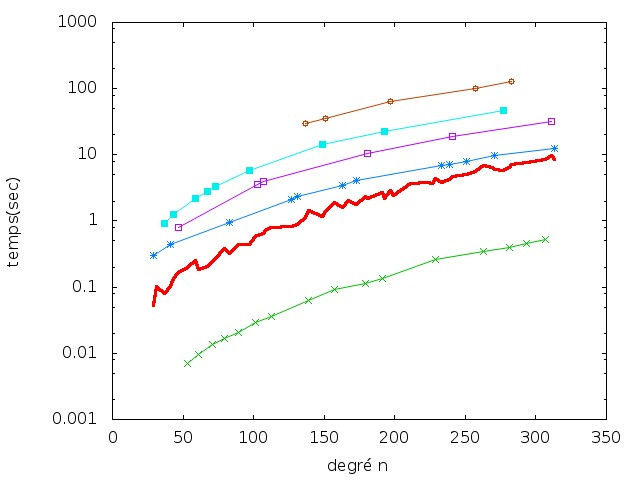
\includegraphics[scale=0.5]{testrc3}
\caption*{ Comparaison de la méthode elliptique
(\textcolor{elliptique}{$\small\blacksquare$}) avec la méthode cyclotomique 
$o = 1$ (\textcolor{o1}{$\times$}), $o = 2$ (\textcolor{o2}{$*$}), $o = 3$ 
(\textcolor{o3}{$\Box$}), $o = 4$ (\textcolor{o4}{$\blacksquare$}), $o = 6$ 
(\textcolor{o6}{$\diamond$}) en fonction du degré $n$, pour $p = 101$}
\end{center}
\end{figure}

\end{frame}
\begin{frame}
\frametitle{Comparaison}
\begin{figure}
\begin{center}
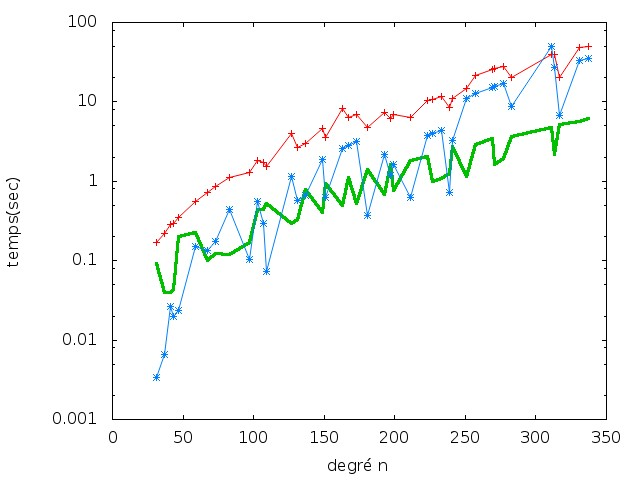
\includegraphics[scale=0.5]{data_test8_ext_flint11}
\caption*{Comparaison de la méthode elliptique (\textcolor{o1}{$\blacksquare$})
avec la méthode naïve (\textcolor{elliptique}{$+$}) et la méthode
Lenstra/Allombert (\textcolor{o2}{$*$}) en fonction du degré $n$, pour $p = 101
$}
\end{center}
\end{figure}
\end{frame}




\section{Conclusion}
\begin{frame}
\frametitle{Conclusion}
\textbf{Résultats :}
\begin{itemize}
	\item Étude et implantation d'un nouvel algorithme;
	\item Résultats compétitifs.
\end{itemize}
\vspace{0.3cm}
\textbf{Futurs objectifs :}
\begin{itemize}
	\item Cas général ($q$ puissance d'un nombre premier, $n$ et $m$ composés);
	\item Possible intégration dans \bsc{SAGE}.
\end{itemize}
\end{frame}
\begin{frame}[plain,c]
%\frametitle{A first slide}

\begin{center}
\Huge Questions ?
\end{center}

\end{frame}
\end{document}
